\section{Implementation}
\label{Imp}



\subsection{Data Plane}

We implement our data plane based on contiki-ng, a system for next generation IoT (Internet of
Things), We modify the network layer of contiki-ng, and abstract
data plane interface to separate network control functions from data plane. 
The details are described as follows.

\textbf{Neighbor Discovery}: After deployment, nodes frist start IPv6 neighbor
discovery protocol to find the nodes which can be reached within one hop, and
then save the neighbor information to neighbor table and wait for UAV arriving
to gather the topology information. Every neighbor's information consists of the
neighbor's IP and RSSI. 

\textbf{Packet Forwarding and Data Sampling}: The nodes get routing table from UAV through
northbound interface. When a node receive a data packet from other nodes, it
just sends it to the next hop node according the routing table. Nodes read task
table received from UAV to decide when to start data sampling to make sure 
that they cost minimal energy to get the same
quality data. 

\subsection{Control Plane}

We run our SDN control plane on a power airborne computer carried by UAV. 
The UAV's flight controller runs on ROS (Robot Operating System) base on UAV's SDK.
And we use MySQL as our SDN database. UAV gathers topology from each node and save
it into database, so that users can easily read the whole network data from
database. For the same reason, after a user gets routing algorithm results and
saves it into database via northbound interface, our control plane will
automatically divides the whole network routing results into individual node's
routing table, and then sends it to specific nodes.

\subsection{Hardware Platform}

Based on our software framework, we use DJI M100 UAV carrying Nvidia TX-2 airborne
computer, and adapt 250 TI CC2650 SensorTag to build our testbed. The TX-2 built around an NVIDIA GPU 
and loaded with 8 GB of memory and 59.7 GB/s of memory bandwidth. It is most power-efficient embedded 
AI computing device which is suitable for UAV onboard computing. The SensorTag communicate with UAV and
other nodes through Zigbee stack, it also equipped with 10 different types of sensors which is suitable for 
large scale wireless sensor networks.

\begin{figure}[htbp]
	\centering
	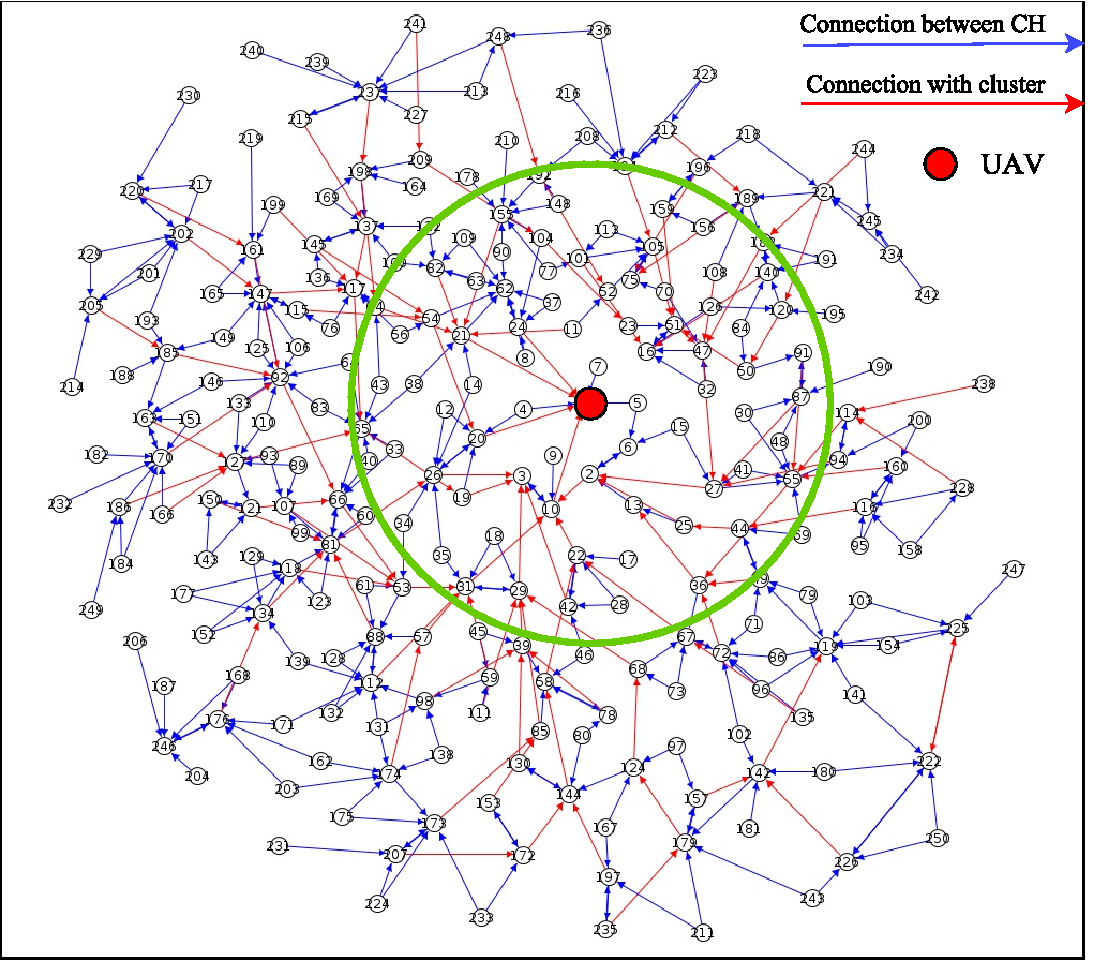
\includegraphics[width=.85\columnwidth]{Figure/topology}
	\vspace{-0.1in}
	\caption{Network Run-time Topology Computed by {\sdn}. \textnormal{The blue lines
represent the connection between cluster members with cluster headers, and the
red lines donate the route between cluster headers deployed by UAV.}}
	
	\label{topology}
	\vspace{-0.1in}
\end{figure}

According to our UAV gathered network run-time topology, we draw Figure~\ref{topology}, the network run-time topology computed by {\sdn}.

